\PassOptionsToPackage{unicode=true}{hyperref} % options for packages loaded elsewhere
\PassOptionsToPackage{hyphens}{url}
%
\documentclass[]{article}
\usepackage{lmodern}
\usepackage{amssymb,amsmath}
\usepackage{ifxetex,ifluatex}
\usepackage{fixltx2e} % provides \textsubscript
\ifnum 0\ifxetex 1\fi\ifluatex 1\fi=0 % if pdftex
  \usepackage[T1]{fontenc}
  \usepackage[utf8]{inputenc}
  \usepackage{textcomp} % provides euro and other symbols
\else % if luatex or xelatex
  \usepackage{unicode-math}
  \defaultfontfeatures{Ligatures=TeX,Scale=MatchLowercase}
\fi
% use upquote if available, for straight quotes in verbatim environments
\IfFileExists{upquote.sty}{\usepackage{upquote}}{}
% use microtype if available
\IfFileExists{microtype.sty}{%
\usepackage[]{microtype}
\UseMicrotypeSet[protrusion]{basicmath} % disable protrusion for tt fonts
}{}
\IfFileExists{parskip.sty}{%
\usepackage{parskip}
}{% else
\setlength{\parindent}{0pt}
\setlength{\parskip}{6pt plus 2pt minus 1pt}
}
\usepackage{hyperref}
\hypersetup{
            pdftitle={Era's CV},
            pdfauthor={Pande Putu Erawijantari},
            pdfborder={0 0 0},
            breaklinks=true}
\urlstyle{same}  % don't use monospace font for urls
\usepackage[margin=1in]{geometry}
\usepackage{graphicx,grffile}
\makeatletter
\def\maxwidth{\ifdim\Gin@nat@width>\linewidth\linewidth\else\Gin@nat@width\fi}
\def\maxheight{\ifdim\Gin@nat@height>\textheight\textheight\else\Gin@nat@height\fi}
\makeatother
% Scale images if necessary, so that they will not overflow the page
% margins by default, and it is still possible to overwrite the defaults
% using explicit options in \includegraphics[width, height, ...]{}
\setkeys{Gin}{width=\maxwidth,height=\maxheight,keepaspectratio}
\setlength{\emergencystretch}{3em}  % prevent overfull lines
\providecommand{\tightlist}{%
  \setlength{\itemsep}{0pt}\setlength{\parskip}{0pt}}
\setcounter{secnumdepth}{0}
% Redefines (sub)paragraphs to behave more like sections
\ifx\paragraph\undefined\else
\let\oldparagraph\paragraph
\renewcommand{\paragraph}[1]{\oldparagraph{#1}\mbox{}}
\fi
\ifx\subparagraph\undefined\else
\let\oldsubparagraph\subparagraph
\renewcommand{\subparagraph}[1]{\oldsubparagraph{#1}\mbox{}}
\fi

% set default figure placement to htbp
\makeatletter
\def\fps@figure{htbp}
\makeatother


\title{Era's CV}
\author{Pande Putu Erawijantari}
\date{2019-12-22}

\begin{document}
\maketitle

\hypertarget{aside}{%
\section{Aside}\label{aside}}

\begin{figure}
\centering
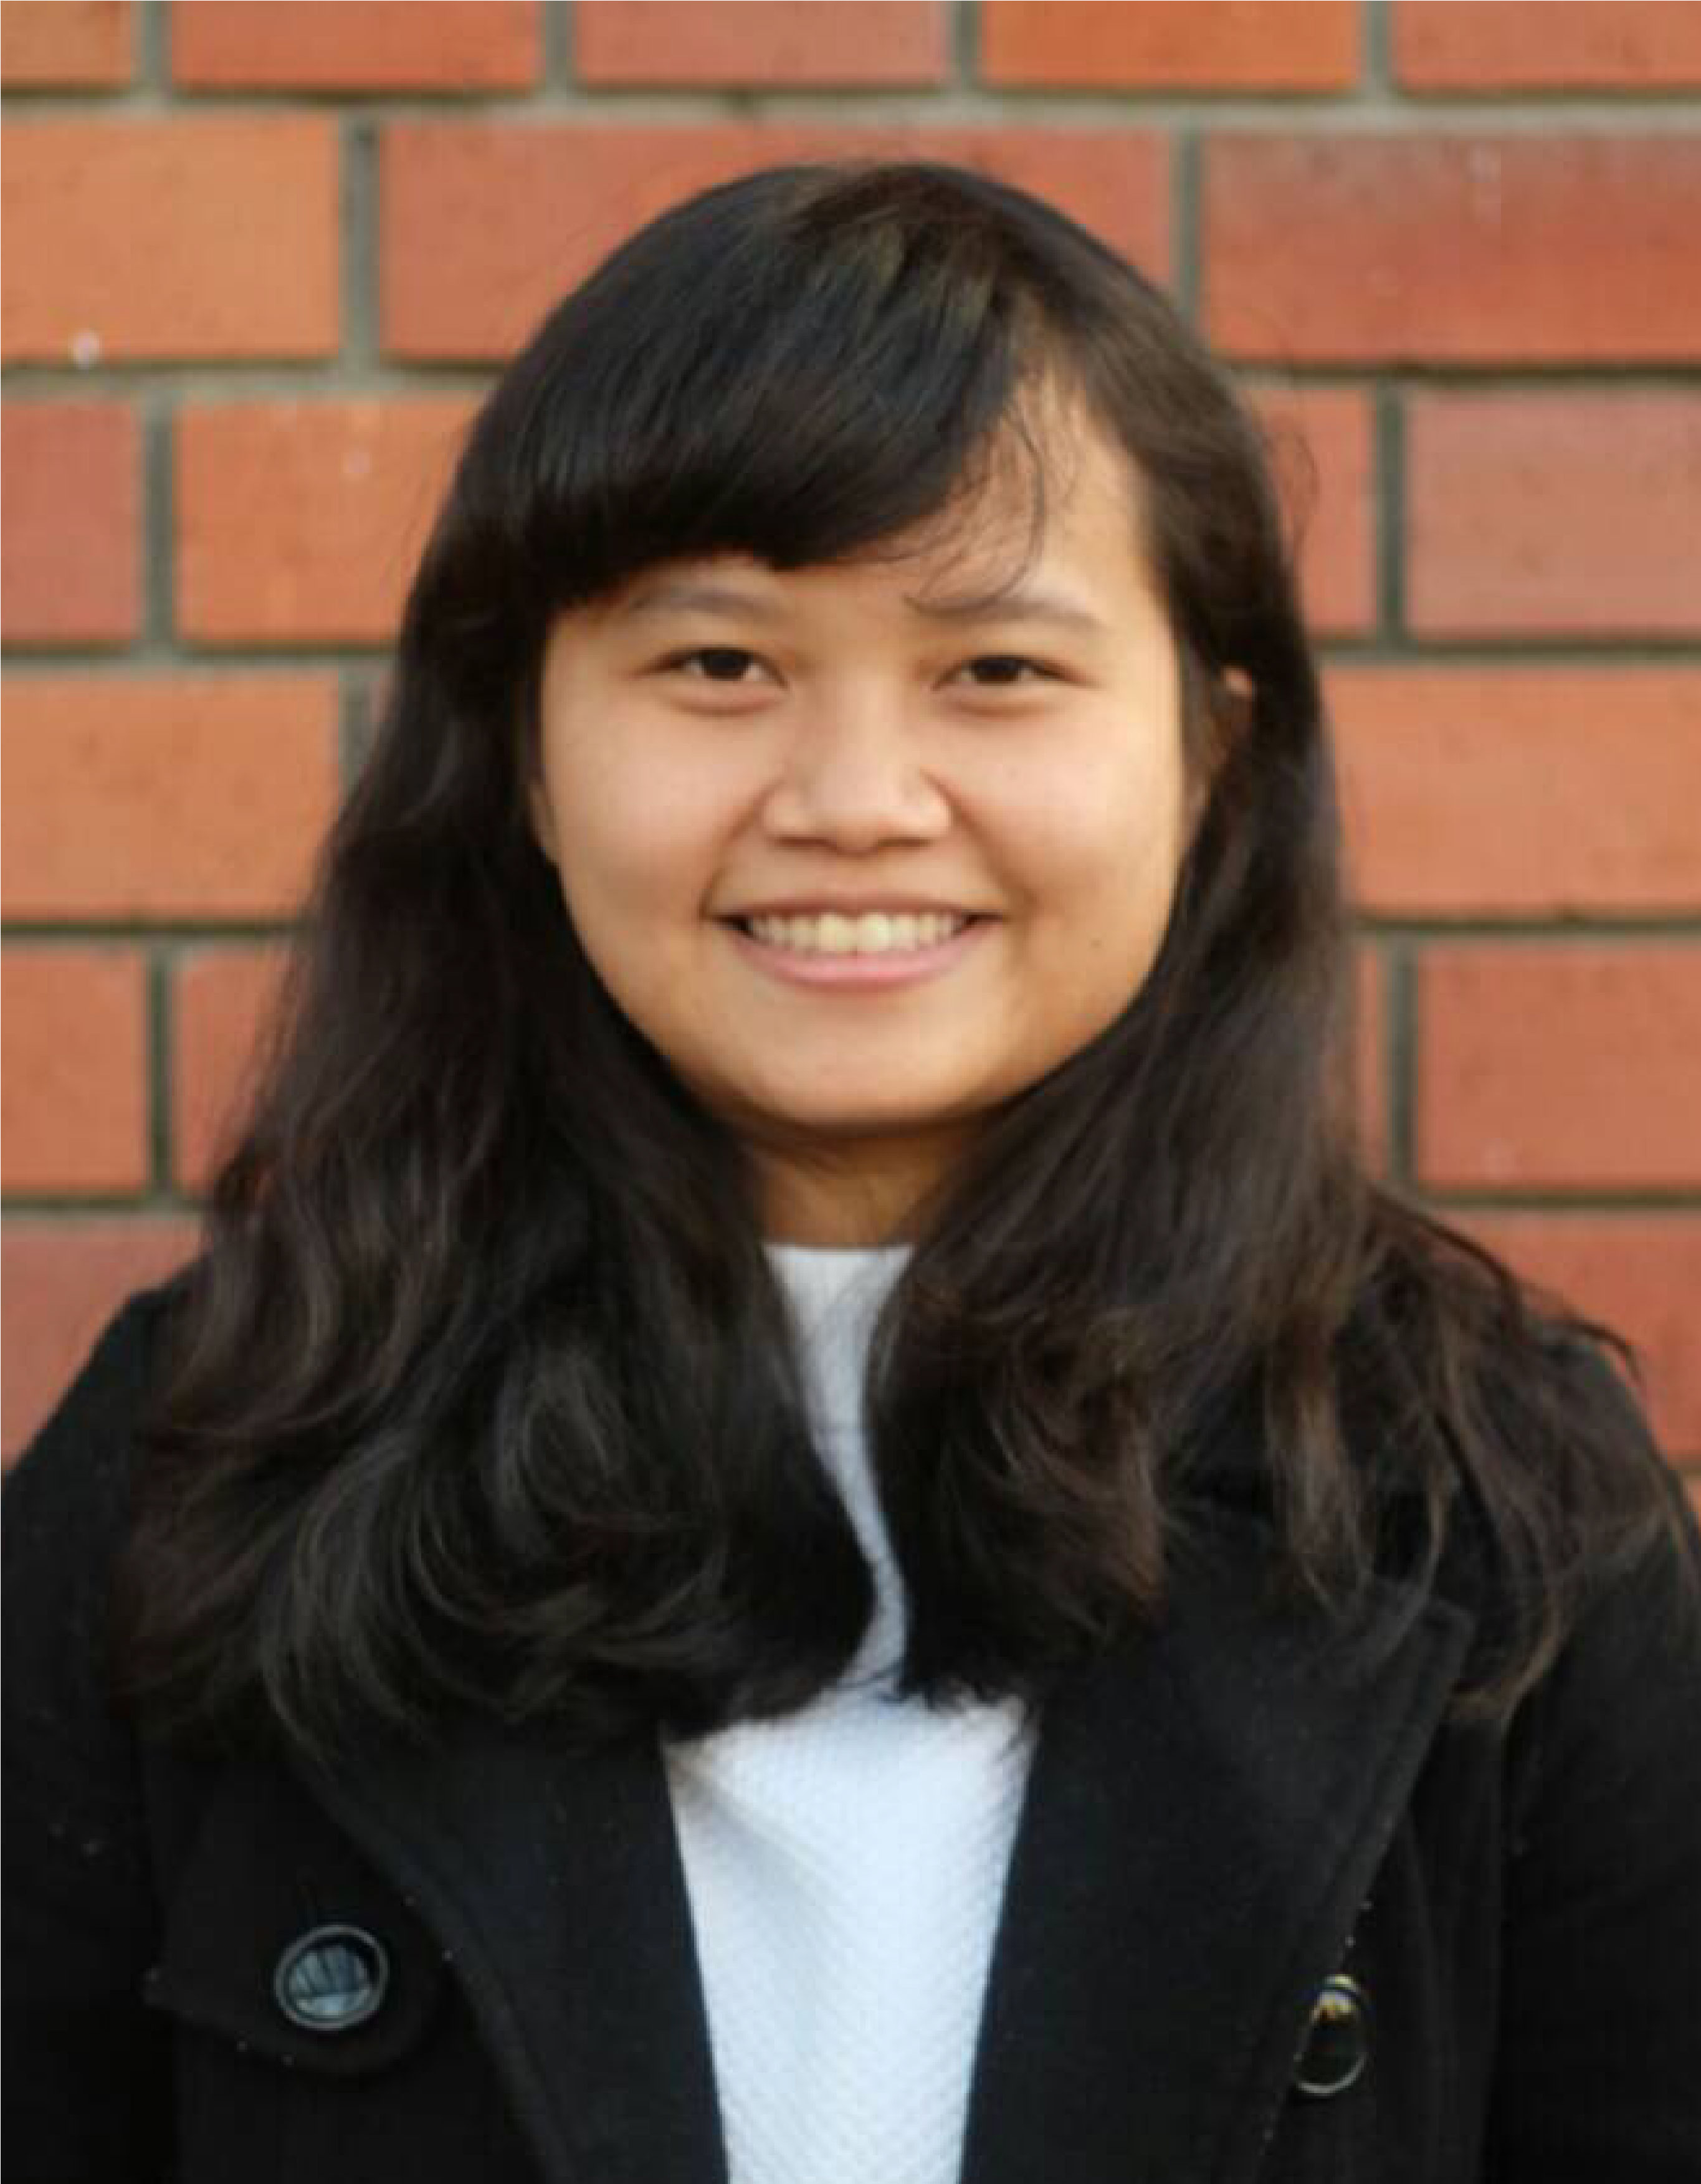
\includegraphics[width=1\textwidth,height=\textheight]{era_fig.jpg}
\caption{logo}
\end{figure}

\hypertarget{contact}{%
\subsection{Contact}\label{contact}}

\begin{itemize}
\tightlist
\item

  \href{mailto:erawijantari@gmail.com}{\nolinkurl{erawijantari@gmail.com}}
\item

  \href{mailto:erawijantari.p.aa@m.titech.ac.jp}{\nolinkurl{erawijantari.p.aa@m.titech.ac.jp}}
\item
   @erawijantaript
\item
   github.com/erawijantari
\item
   \url{erawijantari.github.io}
\item
   +81 3-5734-3591
\end{itemize}

\hypertarget{skills}{%
\subsection{Skills}\label{skills}}

 \texttt{Python}

 \texttt{R}

 \texttt{Git}

 \texttt{Bash}

 \texttt{Unix/Linux}

 \texttt{HPC\ (SGE)}

Experienced in computational bioinformatics and biostatistics applied
for next-generation sequencing data integrated to other omics analysis
especially for microbiome study.

\hypertarget{disclaimer}{%
\subsection{Disclaimer}\label{disclaimer}}

This resume was made with the R package
\href{https://github.com/rstudio/pagedown}{\textbf{pagedown}}.\\

Source code available at:
\href{https://github.com/danangcrysnanto/cv}{github.com/erawijantari/erawijantari.github.io/static/cv}.

Last updated on 2019-12-22.

\hypertarget{main}{%
\section{Main}\label{main}}

\hypertarget{title}{%
\subsection{Pande Putu Erawijantari}\label{title}}

 Interested in applying bioinformatics analysis on the complex
multi-omics data. Current research mainly focus on the dynamics of human
gut microbiome in the gastrointestinal-related diseases and its
association to the treatmnet effectiveness.\\

\hypertarget{education}{%
\subsection{Education}\label{education}}

\hypertarget{phd-candidate-life-science-and-technology}{%
\subsubsection{PhD Candidate-Life Science and
Technology}\label{phd-candidate-life-science-and-technology}}

Tokyo Institute of Technology

Tokyo JP

Present - 2017

\begin{itemize}
\tightlist
\item
  \textbf{Research project}: Gut microbiome in gastrointestinal related
  diseases
\item
  \textbf{Skills learned}: Metagenomics analysis pipeline, Biostatistic,
  Machine learning
\end{itemize}

\hypertarget{m.sc-biological-information}{%
\subsubsection{M.Sc-Biological
Information}\label{m.sc-biological-information}}

Tokyo Institute of Technology

Tokyo JP

2017 - 2015

\begin{itemize}
\tightlist
\item
  \textbf{Research project}: Multi-omics analysis gut microbiome
\item
  \textbf{Skills learned}: Metagenomics analysis pipeline, Biostatistic
\end{itemize}

\hypertarget{b.sc-biology}{%
\subsubsection{B.Sc-Biology}\label{b.sc-biology}}

Institut Teknologi Bandung

Bandung ID

2014 - 2010

\begin{itemize}
\tightlist
\item
  \textbf{Research project}: Gene mutagenesis isolated from deep sea
  metagenome
\item
  \textbf{Skills learned}: Site-directed mutagenesis, Genetic
  engineering, Protein expression, Enzyme kinetic
\end{itemize}

\hypertarget{selected-publications}{%
\subsection{Selected Publications}\label{selected-publications}}

\hypertarget{influence-of-gastrectomy-for-gastric-cancer-treatment-on-faecal-microbiome-and-metabolome-profiles}{%
\subsubsection{\texorpdfstring{\textbf{Influence of gastrectomy for
gastric cancer treatment on faecal microbiome and metabolome
profiles}}{Influence of gastrectomy for gastric cancer treatment on faecal microbiome and metabolome profiles}}\label{influence-of-gastrectomy-for-gastric-cancer-treatment-on-faecal-microbiome-and-metabolome-profiles}}

\textbf{Erawijantari PP}, Mizutani S, Shiroma H, Shiba S, Nakajima T,
Sakamoto T, Saito Y, Fukuda S , Yachida S, Yamada T. \emph{Gut}.
In-press.

N/A

2019

\hypertarget{anti-inflammatory-effect-of-mangosteen-garcinia-mangostana-l.-peel-extract-and-its-compounds-in-lps-induced-raw264.7-cell}{%
\subsubsection{\texorpdfstring{\textbf{Anti-inflammatory effect of
mangosteen (Garcinia mangostana L.) peel extract and its compounds in
LPS-induced RAW264.7
cell}}{Anti-inflammatory effect of mangosteen (Garcinia mangostana L.) peel extract and its compounds in LPS-induced RAW264.7 cell}}\label{anti-inflammatory-effect-of-mangosteen-garcinia-mangostana-l.-peel-extract-and-its-compounds-in-lps-induced-raw264.7-cell}}

Widowati W, Darsono L, Suherman J, Fauziah N, Maesaroh M,
\textbf{Erawijantari PP}. \emph{Nat Prod Sci} 22(3):147-153.

N/A

2016

\hypertarget{in-vitro-study-of-myristica-fragrans-seed-nutmeg-ethanolic-extract-and-quercetin-compound-as-anti-inflammatory-agent}{%
\subsubsection{\texorpdfstring{\textbf{In vitro study of Myristica
fragrans seed (Nutmeg) ethanolic extract and quercetin compound as
anti-inflammatory
agent}}{In vitro study of Myristica fragrans seed (Nutmeg) ethanolic extract and quercetin compound as anti-inflammatory agent}}\label{in-vitro-study-of-myristica-fragrans-seed-nutmeg-ethanolic-extract-and-quercetin-compound-as-anti-inflammatory-agent}}

Dewi K, Widyarto B, \textbf{Erawijantari PP}, Widowati W. \emph{Int J
Res Med Sci} 3 (9), 2303-2310.

N/A

2015

\hypertarget{selected-conference}{%
\subsection{Selected conference}\label{selected-conference}}

\hypertarget{fecal-microbiome-and-metabolome-characterizations-of-patients-after-gastrectomy-for-gastric-cancer-treatment}{%
\subsubsection{\texorpdfstring{\textbf{Fecal microbiome and metabolome
characterizations of patients after gastrectomy for gastric cancer
treatment}}{Fecal microbiome and metabolome characterizations of patients after gastrectomy for gastric cancer treatment}}\label{fecal-microbiome-and-metabolome-characterizations-of-patients-after-gastrectomy-for-gastric-cancer-treatment}}

\textbf{Erawijantari PP}, Mizutani S, Shiroma H, Yachida S, Yamada T.
Keystone Symposia on Molecular and Cellular Biology: Microbiome:
Therapeutic Implications (T1).\textbf{Poster}.

N/A

October, 2019

\hypertarget{metagenomic-and-metabolomic-profiling-to-characterize-the-effect-of-gastrectomy-as-gastric-cancer-treatment-on-human-gut-microbiome}{%
\subsubsection{\texorpdfstring{\textbf{Metagenomic and metabolomic
profiling to characterize the effect of gastrectomy as gastric cancer
treatment on human gut
microbiome}}{Metagenomic and metabolomic profiling to characterize the effect of gastrectomy as gastric cancer treatment on human gut microbiome}}\label{metagenomic-and-metabolomic-profiling-to-characterize-the-effect-of-gastrectomy-as-gastric-cancer-treatment-on-human-gut-microbiome}}

\textbf{Erawijantari PP}, Mizutani S, Shiroma H, Yachida S, Yamada T.
7th International Human Microbiome Consortium : Translating microbiome
science. \textbf{Poster}.

N/A

June, 2018

\begin{itemize}
\tightlist
\item
  \emph{Selected as Early Career Scientist Bursary Recipient}
\end{itemize}

\hypertarget{selected-awards}{%
\subsection{Selected awards}\label{selected-awards}}

\hypertarget{japanese-government-monbukagakushomext-scholarship-recipient}{%
\subsubsection{\texorpdfstring{\textbf{Japanese Government
(Monbukagakusho:MEXT) Scholarship
recipient}}{Japanese Government (Monbukagakusho:MEXT) Scholarship recipient}}\label{japanese-government-monbukagakushomext-scholarship-recipient}}

Awarded to foreign students who study in higher education institutions,
selected on the recommendation of Japanese Embassy/Consulate General,
University, or Authority.

N/A

2020 - 2015

\hypertarget{international-human-microbiome-consortium-2018-early-career-scientist-bursary-recipient}{%
\subsubsection{\texorpdfstring{\textbf{International Human Microbiome
Consortium 2018 Early Career Scientist Bursary
Recipient}}{International Human Microbiome Consortium 2018 Early Career Scientist Bursary Recipient}}\label{international-human-microbiome-consortium-2018-early-career-scientist-bursary-recipient}}

Conference travel grant and available to 12 scientists works on human
microbiome research.

N/A

2018

\hypertarget{gold-medalist-as-itb_indonesia-team-on-igem-international-genetically-engineered-machine}{%
\subsubsection{\texorpdfstring{\textbf{Gold medalist as ITB\_Indonesia
team on iGEM (International Genetically Engineered
Machine)}}{Gold medalist as ITB\_Indonesia team on iGEM (International Genetically Engineered Machine)}}\label{gold-medalist-as-itb_indonesia-team-on-igem-international-genetically-engineered-machine}}

The project title: Ecoliplaster :cell biocatalyst for PET plastic
degradation using E. coli

N/A

2014

\hypertarget{work-experience}{%
\subsection{Work experience}\label{work-experience}}

\hypertarget{reference}{%
\section{REFERENCE}\label{reference}}

\textbf{TAKUJI YAMADA} Associate Professor School of Life Science and
Technology Tokyo Institute of Technology, Tokyo, Japan +813-5734-3629,
\href{mailto:takuji@bio.titech.ac.jp}{\nolinkurl{takuji@bio.titech.ac.jp}}

\hypertarget{student-intern-data-analyst}{%
\subsubsection{\texorpdfstring{\textbf{Student Intern-Data
Analyst}}{Student Intern-Data Analyst}}\label{student-intern-data-analyst}}

METABOLOGENOMICS, INC.

Tokyo JP

Present - 2018

\begin{itemize}
\tightlist
\item
  Contribute as data analyst and metagenomic pipeline development
\end{itemize}

\hypertarget{research-assistant}{%
\subsubsection{\texorpdfstring{\textbf{Research
Assistant}}{Research Assistant}}\label{research-assistant}}

Yamada Laboratory-Tokyo Institute of Technology

Tokyo JP

Present - 2017

\begin{itemize}
\tightlist
\item
  Contribute to methods development for the eukaryotic fraction
  detection and metagenomics analysis pipeline
\end{itemize}

\hypertarget{research-scientist}{%
\subsubsection{\texorpdfstring{\textbf{Research
Scientist}}{Research Scientist}}\label{research-scientist}}

Biomolecular and Biomedical Research Center, Aretha Medika Utama

Bandung ID

2015 - 2014

\begin{itemize}
\tightlist
\item
  Carried out analyses on the phytochemical bioactive screening and the
  potential of Mesenchymal Stem Cells for cancer treatment using human
  cells line model.
\end{itemize}

\hypertarget{on-job-training}{%
\subsubsection{\texorpdfstring{\textbf{On Job
Training}}{On Job Training}}\label{on-job-training}}

Environmental Affairs Department, PT Newmont Nusa Tenggara

Sumbawa ID

2013

\begin{itemize}
\tightlist
\item
  Participated in the environmental assessment as the results of mining
  process and propose the solutions based on the analysis.
\end{itemize}

\end{document}
